%This is a very basic  BE PROJECT PRELIMINARY Report template.

%############################################# 
%#########Author :  PROJECT###########
%#########COMPUTER ENGINEERING############


\documentclass[oneside,a4paper,12pt]{report}
%\usepackage{showframe}
%\hoffset = 8.9436619718309859154929577464789pt
%\voffset = 13.028169014084507042253521126761pt

\fancypagestyle{plain}{%
  \fancyhf{}
  \fancyfoot[CE]{MODERN EDUCATION SOCIETY'S COLLEGE OF ENGINEERING, Department of Computer Engineering 2022}
  \fancyfoot[RE]{\thepage}
}
\pagestyle{fancy}
\fancyhead{}
\renewcommand{\headrulewidth}{0pt}
\footskip = 0.625in
\cfoot{}
\rfoot{}

\usepackage[]{hyperref}
\usepackage{tikz}
\usetikzlibrary{arrows,shapes,snakes,automata,backgrounds,petri}

\usepackage{tabularx}
\usepackage[section]{placeins}
\usepackage[nottoc,notlot,notlof,numbib]{tocbibind}
\usepackage[titletoc]{appendix}
\usepackage{titletoc}
\renewcommand{\appendixname}{Annexure}
\renewcommand{\bibname}{References}

\setcounter{secnumdepth}{5}
\graphicspath{ {./Image/} }
\usepackage{float}
\usepackage{subcaption}
\usepackage{multirow}

\usepackage[ruled,vlined]{algorithm2e}

\begin{document}

\setlength{\parindent}{0mm}
\begin{center}
{\bfseries SAVITRIBAI PHULE PUNE UNIVERSITY \\}
 \vspace*{1\baselineskip}
{\bfseries A PROJECT REPORT ON \\}
 \vspace*{2\baselineskip}
{\bfseries \fontsize{16}{12} \selectfont BE PROJECT TITLE \\ \vspace*{2\baselineskip}}
{\fontsize{12}{12} \selectfont SUBMITTED TOWARDS THE
 \\PARTIAL FULFILLMENT OF THE REQUIREMENTS FOR THE AWARD OF THE DEGREE \\

\vspace*{2\baselineskip}}
{\bfseries \fontsize{14}{12} \selectfont BACHELOR OF ENGINEERING (Computer
Engineering) \\
\vspace*{1\baselineskip}} 
{\bfseries \fontsize{14}{12} \selectfont BY \\ 
\vspace*{1\baselineskip}} 
Student Name  \hspace{25 mm} Exam No:  \\
Student Name \hspace{25 mm} Exam No:   \\
Student Name \hspace{25 mm} Exam No:  \\
Student Name \hspace{25 mm} Exam No:\\
\vspace*{2\baselineskip}
{\bfseries \fontsize{14}{12} \selectfont Under The Guidance of \\  
\vspace*{2\baselineskip}} 
Prof. Guide Name\\
\includegraphics[width=100pt]{collegelogo.png} \\
{\bfseries \fontsize{14}{12} \selectfont DEPARTMENT OF COMPUTER ENGINEERING \\
College Name \\
College Address \\
\vspace*{1\baselineskip}
Academic Year
}
\end{center}


\newpage



\begin{figure}[ht]
\centering
\includegraphics[width=100pt]{collegelogo.png}
\end{figure}


{\bfseries \fontsize{14}{12} \selectfont \centerline{College Name}
\centerline{DEPARTMENT OF COMPUTER ENGINEERING}
\vspace*{3\baselineskip}} 


{\bfseries \fontsize{16}{12} \selectfont \centerline{CERTIFICATE} 
\vspace*{3\baselineskip}} 

\centerline{This is to certify that the Project Entitled}
\vspace*{1\baselineskip} 


{\bfseries \fontsize{14}{12} \selectfont \centerline{BE PROJECT TITLE}
\vspace*{1\baselineskip}}

\centerline{Submitted by}
\vspace*{1\baselineskip} 
\centerline{Student Name  \hspace{25 mm} Exam No: } 
\centerline{Student Name \hspace{25 mm} Exam No:  } 
\centerline{Student Name \hspace{25 mm} Exam No: }
\centerline{Student Name \hspace{25 mm} Exam No: }
\vspace*{1\baselineskip} 
is a bonafide work carried out by Students under the supervision of Prof. Guide Name and it
is submitted towards the partial fulfillment of the requirement of Savitribai Phule Pune Univercity,Pune for the award of the degree of Bachelor of Engineering (Computer Engineering). Project.\\\\\\
\bgroup
\def\arraystretch{0.7}
\begin{tabular}{c c c}
External Examiner &  \hspace{10 mm} Prof. Guide Name & \hspace{10 mm} Prof. HOD Name \\					     &  \hspace{10 mm} Internal Guide   &  \hspace{10 mm} H.O.D \\
 &  \hspace{10 mm} Dept. of Computer Engg.  &	\hspace{10 mm}Dept. of Computer Engg.  \\
\end{tabular}
%}
\\\\
Date:\\
Place:


\newpage

%\pictcertificate{TITLE OF BE PROJECT}{Student Name}{Exam Seat No}{Guide Name}
\setcounter{page}{0}
\frontmatter
\cfoot{MESCOE, Department of Computer Engineering 2022}
\rfoot{\thepage}
\pagenumbering{Roman}
%\pictack{BE PROJECT TITLE}{Guide Name}

		
{  \newpage {\bfseries \fontsize{14}{12} \selectfont \centerline{Abstract} 
\vspace*{2\baselineskip}} \setlength{\parindent}{11mm} }
{ \setlength{\parindent}{0mm} }
Please Write here One Page Abstract. It should mainly include introduction, motivation,outcome and innovation if any.


{  \newpage {\bfseries \fontsize{14}{12} \selectfont \centerline{Acknowledgments} 
\vspace*{2\baselineskip}} \setlength{\parindent}{11mm} }
{ \setlength{\parindent}{0mm} }
Please Write here Acknowledgment.Example given as\\
\textit{It gives us great pleasure in presenting the preliminary project report 
on {\bfseries \fontsize{12}{12} \selectfont `BE PROJECT TITLE'}.}
\vspace*{1.5\baselineskip}

 \textit{I would like to take this opportunity to thank my internal guide
 \textbf{Prof. Guide Name} for giving me all the help and guidance I needed. I am
 really grateful to them for their kind support. Their valuable suggestions were very helpful.} \vspace*{1.5\baselineskip}

 \textit{I am also grateful to \textbf{Prof. HOD Name}, Head of Computer
 Engineering Department, CollegeName for his indispensable
 support, suggestions.}
\vspace*{1.5\baselineskip}

\textit{In the end our special thanks to \textbf{Other Person Name} for
providing various resources such as  laboratory with all needed software platforms,
continuous Internet connection, for Our Project.}
\vspace*{3\baselineskip} \\
\begin{tabular}{p{8.2cm}c}
&Student Name1\\
&Student Name2\\
&Student Name3\\
&Student Name4\\
&(B.E. Computer Engg.)
%}
\end{tabular}


% \maketitle
\tableofcontents
\listoffigures 
\listoftables



\mainmatter











\setlength{\parindent}{11mm}





\chapter{INTRODUCTION}

        A human gesture can be defined as a sequence of states in the short-lived motion of some part of the body, most commonly the hands and face. Consider the wave of a hand in order to open a door controlled by sensors. The gesture has an initial position and a final position, with many small states in the transition from the initial state to the final state. For example, for a left-to-right wave, the hand is initially at the left, and is moved to the right in a quick and swift movement. This very well explains the meaning of a gesture.
    
    
         Existing techniques of hand gesture recognition can be divided into two broad categories on the basis of method of obtaining input – vision-based techniques and non-vision based techniques. Vision-based techniques usually imply the use of cameras or motion sensors to detect movement and thus extract input. No extra equipment is generally required in this approach. Non-vision based techniques commonly use hardware equipment to extract input, such as wearable devices. These wearable devices are equipped with various types of mechanical or optical sensors, that translate movement of the body part into electrical signals.
    
    
         Vision-based gesture tracking presents itself to be a more practical and feasible measure, since there is no need for the user to have an extra hardware device(e.g. wearable) for motion to be detected – as long as the motion is in the tracking frame of the sensor, it can be taken as an input for gesture recognition.
    
    
         It is quite common knowledge that computer systems and applications can be controlled(or navigated) by the use of remote-like devices that generate signals which are tracked by the system through sensors, and the respective operations are performed by the system. Consider a Playstation Move motion controller for a clearer picture. But what if we could eliminate the need for these physical devices and achieve truly contact-less system control, through mere hand gestures in front of a camera or similar sensors?
     
    \chapter{MOTIVATION}
        Traditional(or conventional) methods of human-computer interaction, namely, keyboards, pointing devices, and similar physical input tools, and the more popular and commonly-used touchscreens, are only as useful through the application of pressure through physical touch.


        The recent pandemic has driven a major argument about the substantial and often, indispensable need for contact-less operation of systems, irrespective of the scale of the industry. Say for example, supply chain systems that are handled by scores of employees in the span of a day. 


        It is quite fundamental knowledge now, that how public systems that work on physical contact can pose as potential vectors for diseases. Hand gesture recognition can turn out to be an excellent solution to this problem; facilitating truly contact-less interaction with computing devices, and at the same time providing dependable and respectable efficiency.


\chapter{PROBLEM DEFINITION}
    To explore various techniques of recognition of hand gestures so as to study a way of efficient human-computer interaction.


    To elaborate on a technique that conforms to our purposes and requirements of classifying a set of pre-determined hand gestures through a video input, i.e., using 2-dimensional convolutions neural networks and long-short term memory network.
    
    
    To configure a way to effectively map the hand gestures classified to a corresponding operation performed in order to achieve basic system control through gestures.




\chapter{LITERATURE SURVEY}
    Zhang, et al. Designed a 3-dimensional convolutions neural network model(CNN) [1], this study applies a deep learning method to recognise hand gestures. 3D Convolution neural network can be seen as a variant of 2D convolution  neural network extending 2dimension filter into 3 dimensions. This 3D filter shall slide in 3 directions to extract low-level features and its output’s shape is a 3dimension space like a cuboid Uses the Jester V1.0 hand gesture dataset to train the model. According to the result of the training experiment, it got an average accuracy of 90%. 
    
    Wang et al. developed temporal segment networks (TSN) in [2], for action recognition. In the TSN model, each input video sample is divided into a number of segments and a short snippet is randomly selected from each segment. The snippets are represented by modalities such as RGB frames, optical flow and RGB differences. Convolutions neural networks (ConvNets) that are used to learn these snippets all share parameters. The class scores of different snippets are fused by the segmental consensus function to yield segmental consensus, which is a video-level prediction. Predictions from all modalities are fused to produce the final prediction. Experiment showed that the model not only achieved very good action recognition accuracy but also maintained reasonable computation cost. 
    Min, et al. [3] formulate gesture recognition as an irregular sequence recognition problem and aim to capture long-term spatial correlations across point cloud sequences. A novel and effective PointLSTM is proposed to propagate information from past to future while preserving the spatial structure. The proposed PointLSTM combines state information from neighboring points in the past with current features to update the current states by a weight-shared LSTM layer. This method can be integrated into many other sequence learning approaches. In the task of gesture recognition, the proposed PointLSTM achieves state-of-the-art results on two challenging datasets (NVGesture and SHREC'17) and outperforms previous skeleton-based methods. To show its advantages in generalization, we evaluate our method on MSR Action3D dataset, and it produces competitive results with previous skeleton-based methods.
    
    Tang, et al. [4] combined image entropy and density clustering to exploit the key frames from hand gesture video for further feature extraction, which can improve the efficiency of recognition. Moreover, a feature fusion strategy is also proposed to further improve feature representation, which elevates the performance of recognition. To validate our approach in a "wild" environment, we also introduce two new datasets called Hand Gesture and Action3D datasets. Experiments consistently demonstrate that our strategy achieves competitive results on Northwestern University, Cambridge, HandGesture and Action3D hand gesture datasets
    Cheng, et al. [5] proposed a Dynamic Graph-Based Spatial-Temporal Attention (DG-STA) method for hand gesture recognition. The key idea is to first construct a fully-connected graph from a hand skeleton, where the node features and edges are then automatically learned via a self-attention mechanism that performs in both spatial and temporal domains. We further propose to leverage the spatial-temporal cues of joint positions to guarantee robust recognition in challenging conditions. In addition, a novel spatial-temporal mask is applied to significantly cut down the computational cost by 99%. We carry out extensive experiments on benchmarks (DHG-14/28 and SHREC'17) and prove the superior performance of our method compared with the state-of-the-art methods.
    Zhang, Wang, Lan [6] Presents a novel deep learning network for hand gesture recognition. The network integrates several well- proved modules together to learn both short-term and long-term features from video inputs and meanwhile avoid intensive computation. To learn short-term features, each video input is segmented into a fixed number of frame groups. A frame is randomly selected from each group and represented as an RGB image as well as an optical flow snapshot. These two entities are fused and fed into a convolutional neural network (ConvNet) for feature extraction. The ConvNets for all groups share parameters. To learn long term features, outputs from all ConvNets are fed into a long short-term memory (LSTM) network, by which a final classification result is predicted. The new model has been tested with two popular hand gesture datasets, namely the Jester dataset and Nvidia dataset. The robustness of the model has also been proved with an augmented dataset with enhanced diversity of hand gestures. Uses the Jester dataset and Nvidia Dataset Achieved an accuracy if around 95%(Jester dataset) and 85%(NVIDIA's dataset).





\chapter{SOFTWARE REQUIREMENT SPECIFICATION}

    \section{Introduction}
        \subsection{Project Scope}
            We trying to build a system which can provide contactless interaction between user and physical hardware of any machine where user need to navigate through the interface like our personal computer, laptop, and ATM machine.
        \subsection{User Classes and Characteristics}
            Users who can perform hand gesture can make use of this system to navigate through the OS without making any physical contact to the physical hardware. User will need to perform meaning or proper gesture to navigate through OS.
        \subsection{Assumptions and Dependencies}
            We are going to assume that user’s machine have already install all the necessary software like .Net frame work, C++ redistribution (2019) and all the necessary driver related to webcam or any optical camera for capturing the user’s gestures.
            
            
            
    \section{Functional Requirements}
        \subsection{Feature vector extraction}
            Feature vector extraction: For feature vector extraction we require the CNN model. For our project we are going to use 2D CNN model for feature extraction. 
        \subsection{Video sequence}
            For video sequence we need the webcam. Which will capture the gesture/moment of user’s hand.
        \subsection{Gesture classification}
            For classification we required RNN model. We will be using LSTM model for gesture classification. 
        \subsection{Mapping gesture to OS operation}
            For Mapping particular gesture to perform OS navigation operation we will need the OpenCV library. 

    
    
    
    \section{External Interface Requirements}
        \subsection{User Interfaces}
        User need to the perform the valid gesture to navigate through operating system. 
        \subsection{Hardware Interface}
        Webcam is required for capturing the video stream of the user who is performing the gesture. And webcam should have recording speed of 30 FPS at least
        \subsection{Software Interface}
        OpenCV is require for mapping the particular gesture to the OS navigation operation. 

    
    
    \section{Nonfunctional Requirements}
        \subsection{Performance Requirement: }
        Video stream should be capture at the speed of 30FPS.
        \subsection{Safety Requirement: }
        No safety related risk are expected.
        \subsection{Security Requirement}
        No user personal data or any image will be saved by the system.
        \subsection{Software quality attributes}
        Usability, Reliability, Portability, Testable, Flexibility.
        
    
    \section{System  Requirements }
        \subsection{Software Requirement}
            \begin{itemize}
        
                \item Operating System: Windows 10.
                \item Programming Language: Python.
                \item Library: OpenCV, TensorFlow, Pandas, Numpy, Keras.
                
    
            \end{itemize}
            \subsection{Hardware Requirement}
                \begin{itemize}
        
                    \item CPU: DUO core (of 4 generation or above).
                    \item Ram: 4GB or above.
                    \item Graphic Card (for training & testing and neural network ): GT 1050 or Intel 520.
                    \item Storage: 500GB HDD or SDD.
                    \item Webcam: should able to recording at 30FPS (Frame Per second).
    
                \end{itemize}
    
    
    \section{Analysis Models: SDLC Model to be applied}
        We will be following the water fall model for our software development life-cycle. The waterfall model is a continuous software development model in which development is seen as flowing steadily downwards (like a waterfall) through the steps of requirements analysis, design, implementation, testing (validation), integration, and maintenance.

Linear ordering of activities has some significant consequences. First, to identify the end of a phase and the beginning of the next, some certification techniques have to be employed at the end of each step. Some verification and validation usually do this mean that will ensure that the output of the stage is consistent with its input (which is the output of the previous step), and that the output of the stage is consistent with the overall requirements of the system.

Phases in Waterfall Model:
\begin{itemize}

  \item Requirements analysis and specification phase: The aim of this phase is to understand the exact requirements of the customer and to document them properly. Both the customer and the software developer work together so as to document all the functions, performance, and interfacing requirement of the software. It describes the "what" of the system to be produced and not "how."In this phase, a large document called Software Requirement Specification (SRS) document is created which contained a detailed description of what the system will do in the common language.
  
  \item Design Phase: This phase aims to transform the requirements gathered in the SRS into a suitable form which permits further coding in a programming language. It defines the overall software architecture together with high level and detailed design. All this work is documented as a Software Design Document (SDD).
  
  \item Implementation and unit testing: During this phase, design is implemented. If the SDD is complete, the implementation or coding phase proceeds smoothly, because all the information needed by software developers is contained in the SDD.
  
  \item Integration and System Testing: This phase is highly crucial as the quality of the end product is determined by the effectiveness of the testing carried out. The better output will lead to satisfied customers, lower maintenance costs, and accurate results. Unit testing determines the efficiency of individual modules. However, in this phase, the modules are tested for their interactions with each other and with the system.
  
  \item Operation and maintenance phase: Maintenance is the task performed by every user once the software has been delivered to the customer, installed, and operational.
\end{itemize}
        
        
    \section{System Implementation Plan}
        \subsection{Objective}  
            \begin{itemize}
                \item Create dataset of video containing different gesture.
                \item Decide mapping of gesture to OS navigation operation.
                \item Setting up development environment.
                \item Create CNN model (for feature extraction).
                \item Create RNN model (for classification).
                \item Create function to execute classified gesture.
                \item Create General overlay for system (UI).
                \item System Integration.
                \item Testing and debugging.

                
            \end{itemize}
            
            \subsection{Outline deliverable}
            Dataset and mapping gesture to navigation operation has to be done in first.
Then only we start creating feature group. Setting up the development environment with all required dependencies.

            \subsection{Tasks}
            
            
            \begin{itemize}
                \item Dataset and mapping gesture.
                \item Setting up development environment.
                \item CNN model development.
                \item RNN model development.
                \item Integration.
                \item Training and testing.
                \item Debugging.
                \item Final tweaking.
                \item Documentation.
                
            \end{itemize}
            
            
            



        




\chapter{SYSTEM DESIGN}

    \section{System Architecture}
        
        \begin{center}
        	\begin{figure}[!hp]
        		\centering
        		\fbox{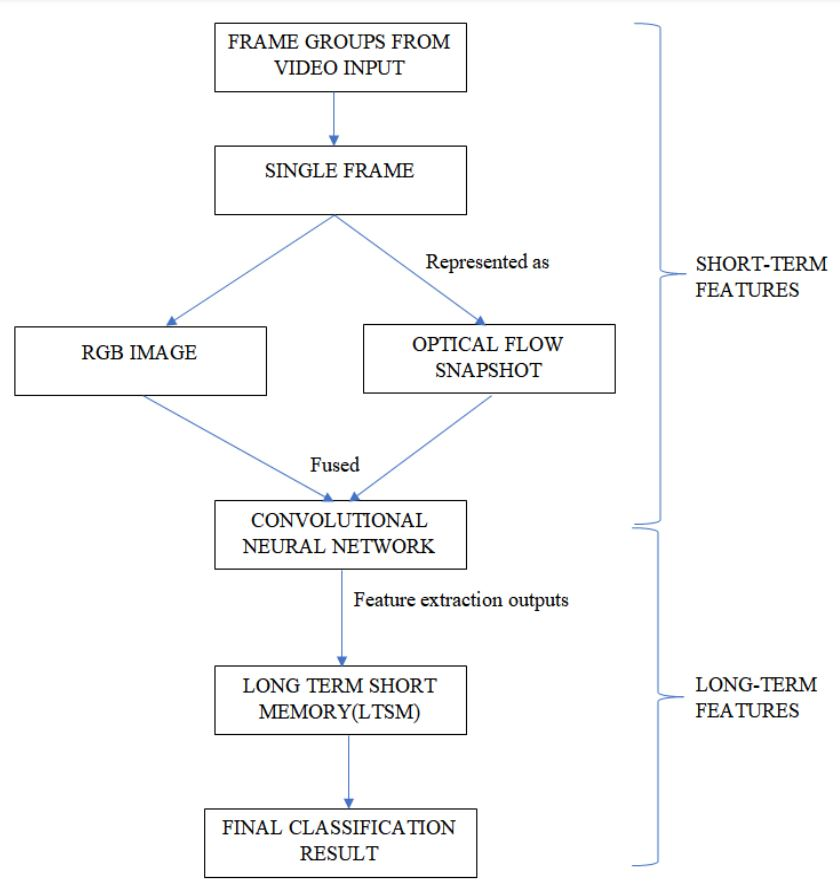
\includegraphics[width=\textwidth]{Architecture.jpg}}
        	  \caption{Architecture diagram}
        	  \label{fig:Architecture}
        	\end{figure}
        \end{center} 
        We will be video stream of user performing the gesture. Then we will be creating the RGB image and Optical flow image using image prepossessing for each image. The RGB and optical flow image will be grouped together and send it to CNN model for feature extraction.
        CNN model will take RGB and optical flow image frame by frame as an input for feature extraction. CNN model will create feature vector groups. 
        
        Feature group are the characteristic of the input provided to the CNN model.
        The feature vector will be taken as the input for RNN model. RNN model are used for classification based on the feature vector group. RNN model will classify the gesture based on the feature vector.
        Based on the classified gesture the particular navigation operation is executed.
    
     \pagebreak
    \section{Data Flow Diagram}
    
        \begin{center}
        	\begin{figure}[!hp]
        		\centering
        		\fbox{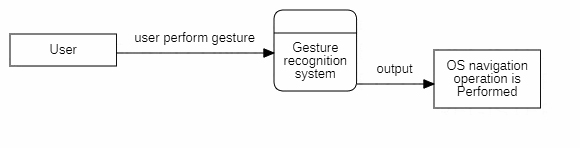
\includegraphics[width=\textwidth]{Image/DFDDiagram1_level_0.jpg}}
        	  \caption{Data flow level 0 diagram}
        	  \label{fig:Data flow level 0}
        	\end{figure}
        \end{center} 
        User will perform gesture. It will be capture by the webcam. video stream in given as input to the system. Then system recognise the gesture and system will perform the related navigation operation to the classified gesture.
        
        \begin{center}
        	\begin{figure}[!hp]
        		\centering
        		\fbox{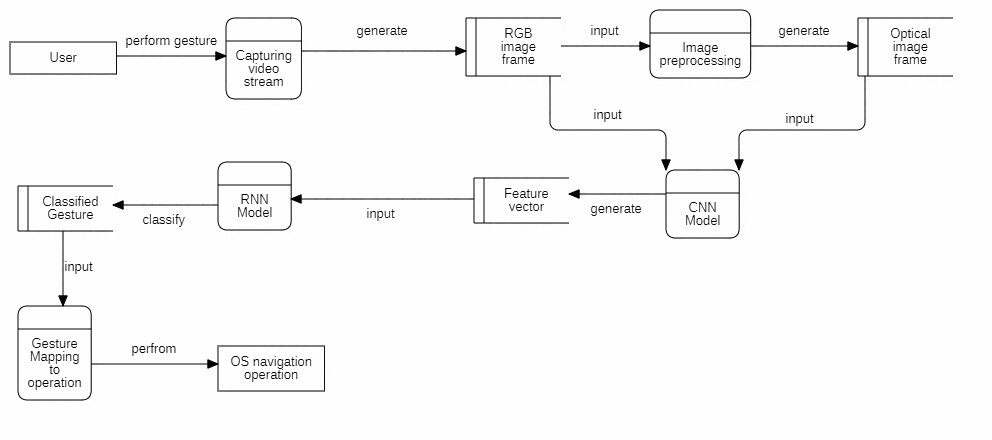
\includegraphics[width=\textwidth]{Image/DFDDiagram1_level_1.jpg}}
        	  \caption{Data flow level 1 diagram}
        	  \label{fig:Data flow level 1}
        	\end{figure}
        \end{center}
        
        \begin{center}
        	\begin{figure}[!hp]
        		\centering
        		\fbox{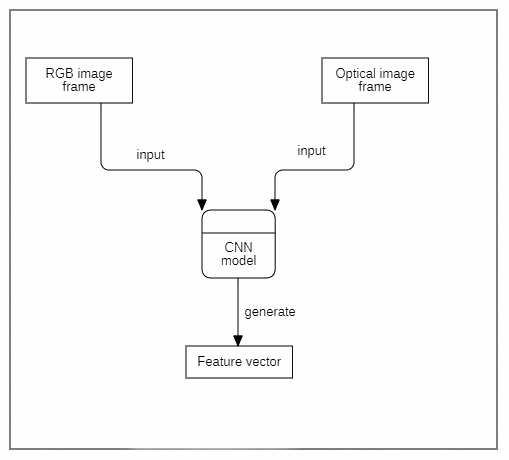
\includegraphics[width=\textwidth]{Image/DFDDiagram1_level_2_1.jpg}}
        	  \caption{Data flow level 2 (1) diagram}
        	  \label{fig:Data flow level 2}
        	\end{figure}
        \end{center}
        
        \begin{center}
        	\begin{figure}[!hp]
        		\centering
        		\fbox{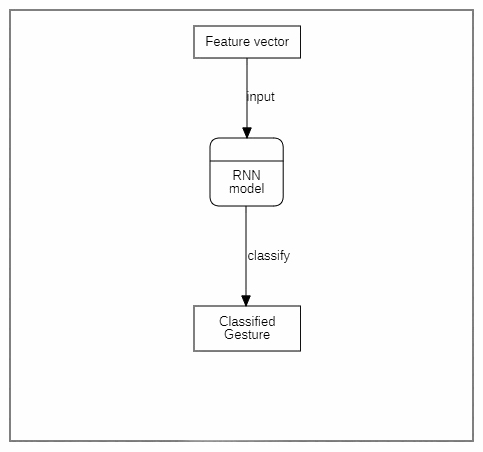
\includegraphics[width=\textwidth]{Image/DFDDiagram1_level_2_2.jpg}}
        	  \caption{Data flow level 2 (2) diagram}
        	  \label{fig:Data flow level 2}
        	\end{figure}
        \end{center}
        
        \begin{center}
        	\begin{figure}[!hp]
        		\centering
        		\fbox{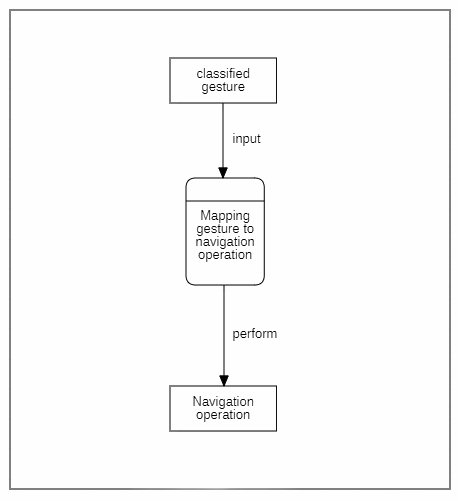
\includegraphics[width=\textwidth]{Image/DFDDiagram1_level_2_3.jpg}}
        	  \caption{Data flow level 2 (2) diagram}
        	  \label{fig:Data flow level 2}
        	\end{figure}
        \end{center}
    
     \pagebreak
    \section{Entity Relationship Diagram}
        \begin{center}
        	\begin{figure}[!hp]
        		\centering
        		\fbox{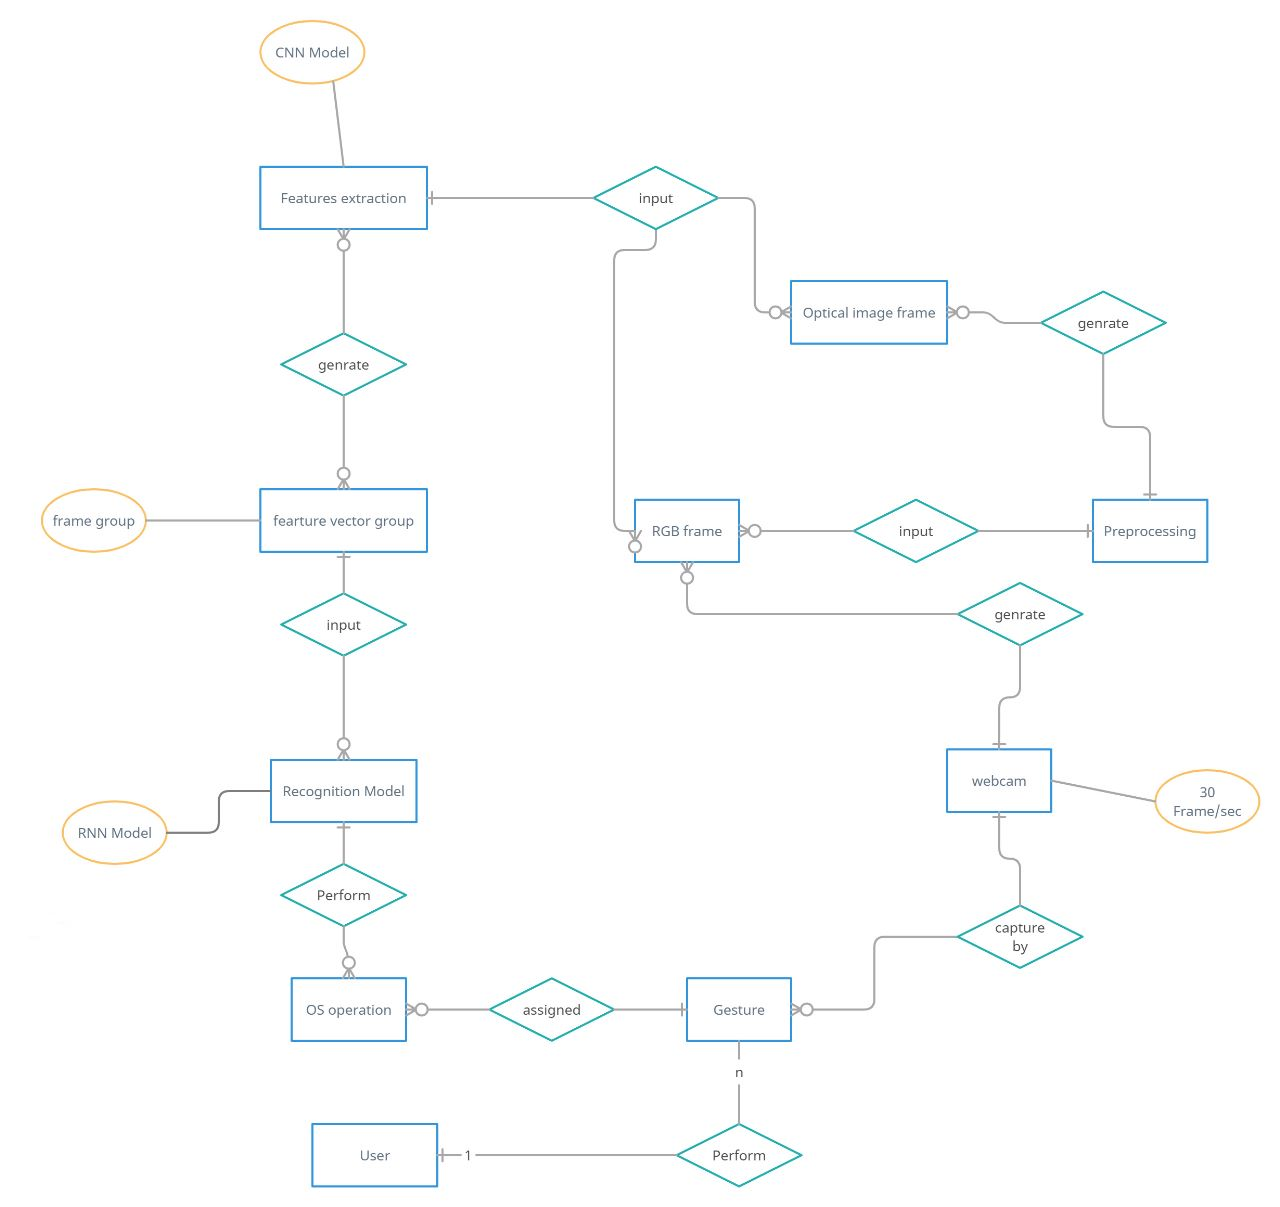
\includegraphics[width=\textwidth]{Image/ERDiagram.jpg}}
        	  \caption{Entity Relationship diagram}
        	  \label{fig:Entity Relationship}
        	\end{figure}
        \end{center}
        
     \pagebreak
    \section{UML Diagrams}
    
     \begin{center}
        	\begin{figure}[!hp]
        		\centering
        		\fbox{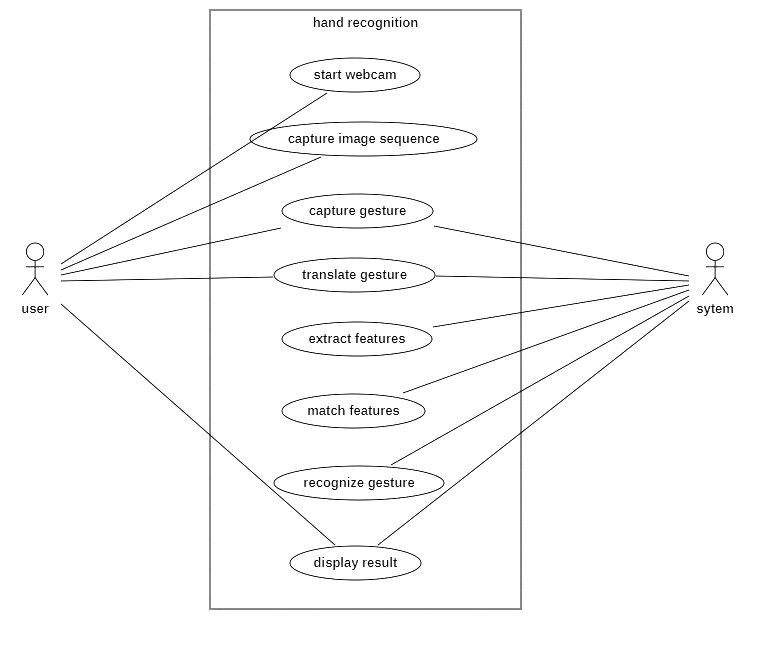
\includegraphics[width=\textwidth]{Image/UseCaseDiagram1.jpg}}
        	  \caption{Use Case diagram}
        	  \label{fig:Use Case}
        	\end{figure}
        \end{center}
        
        \begin{center}
        	\begin{figure}[!hp]
        		\centering
        		\fbox{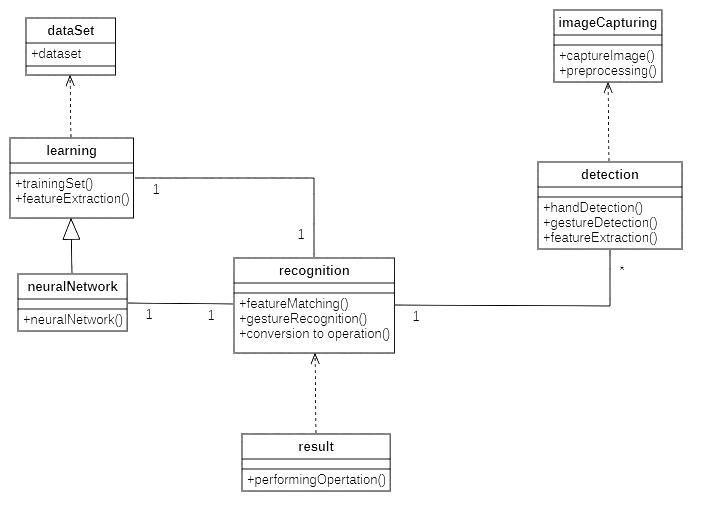
\includegraphics[width=\textwidth]{Image/ClassDiagram1.jpg}}
        	  \caption{Class diagram}
        	  \label{fig:Class diagram}
        	\end{figure}
        \end{center}
        
        \begin{center}
        	\begin{figure}[!hp]
        		\centering
        		\fbox{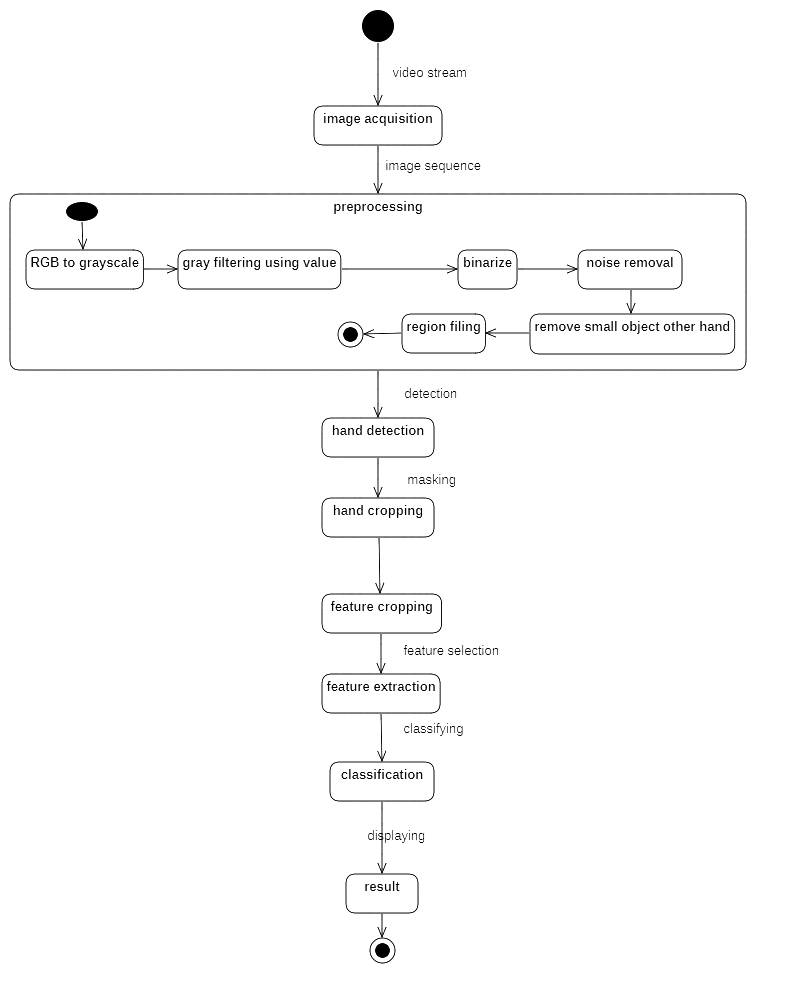
\includegraphics[width=\textwidth]{Image/StatechartDiagram1.jpg}}
        	  \caption{State diagram}
        	  \label{fig:State diagram}
        	\end{figure}
        \end{center}
        
        \begin{center}
        	\begin{figure}[!hp]
        		\centering
        		\fbox{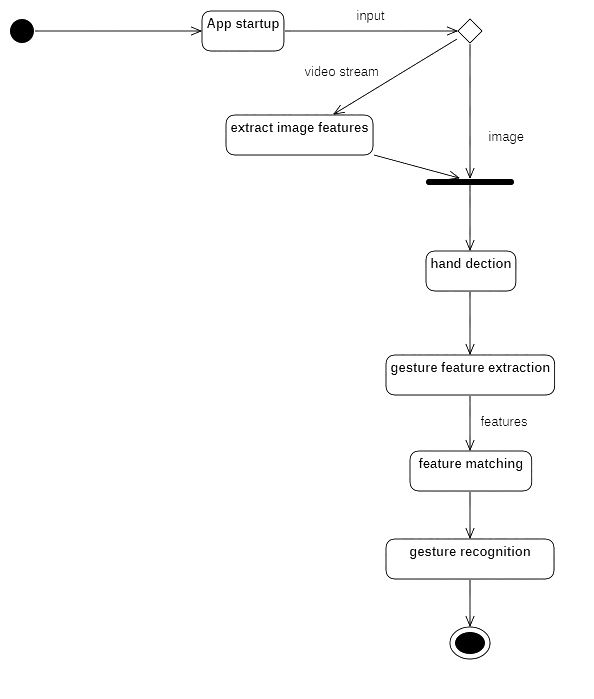
\includegraphics[width=\textwidth]{Image/ActivityDiagram.jpg}}
        	  \caption{Activity diagram}
        	  \label{fig:Activity diagram}
        	\end{figure}
        \end{center}
        
        \begin{center}
        	\begin{figure}[!hp]
        		\centering
        		\fbox{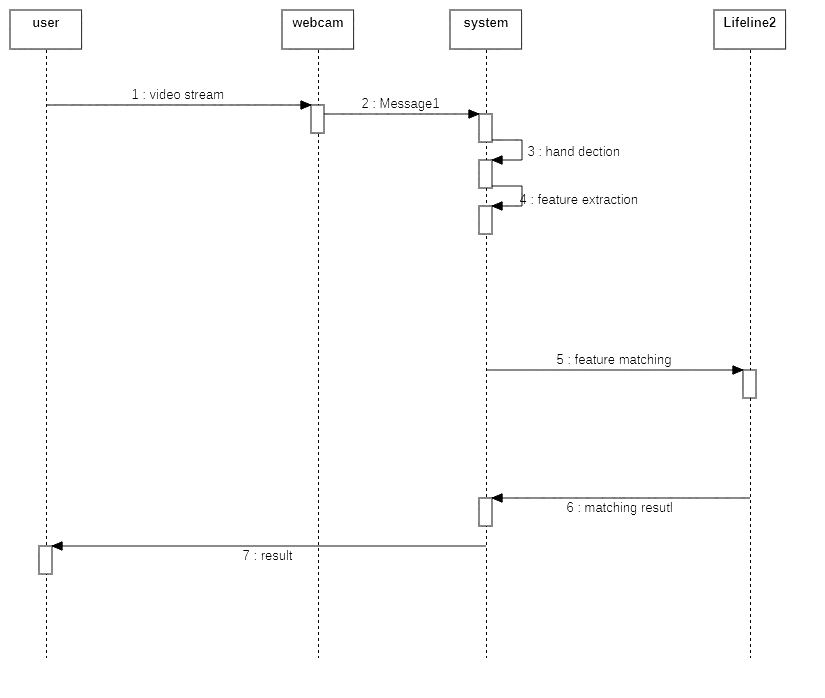
\includegraphics[width=\textwidth]{Image/SequenceDiagram1.jpg}}
        	  \caption{Class diagram}
        	  \label{fig:Class diagram}
        	\end{figure}
        \end{center}
        
        \begin{center}
        	\begin{figure}[!hp]
        		\centering
        		\fbox{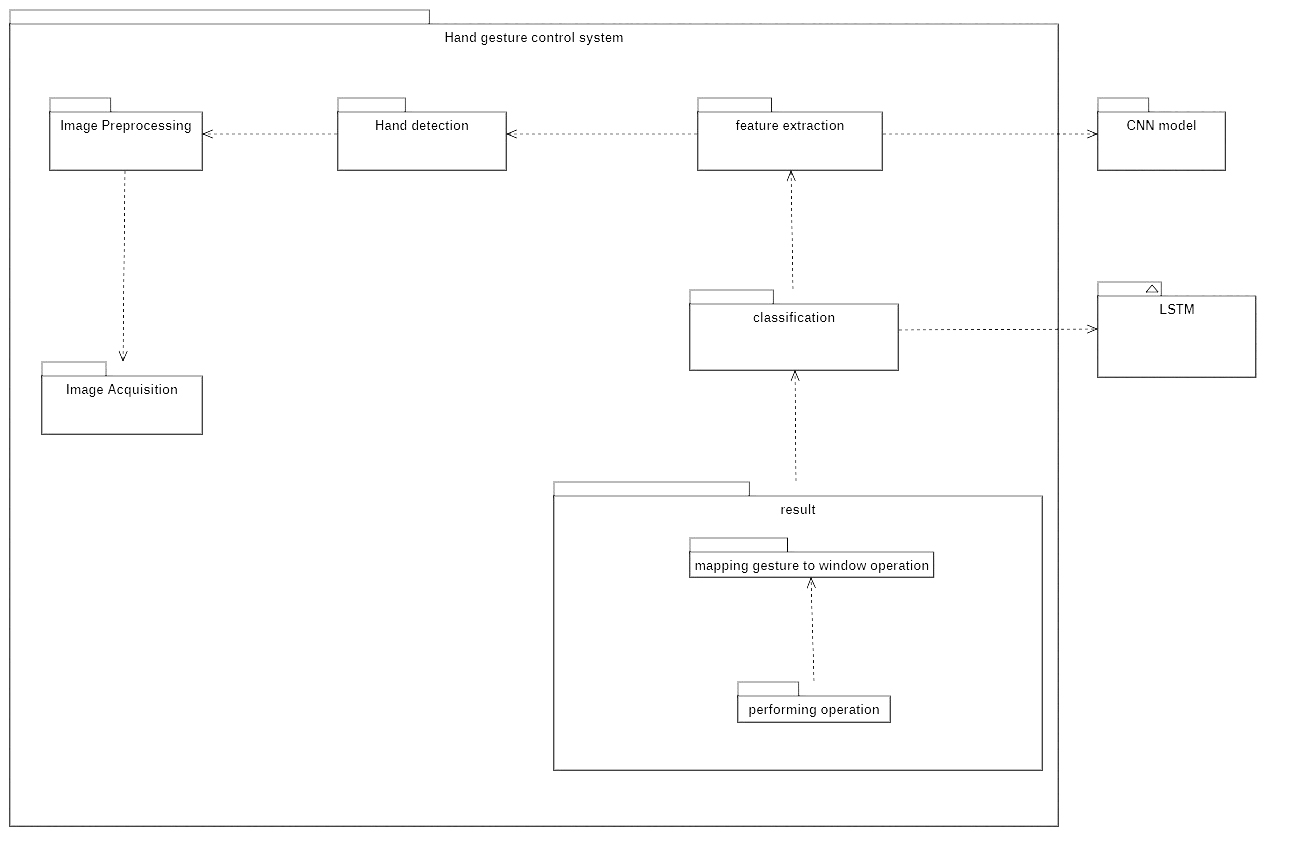
\includegraphics[width=\textwidth]{Image/PackageDiagram1.jpg}}
        	  \caption{Package diagram}
        	  \label{fig:Package diagram}
        	\end{figure}
        \end{center}
        
        \begin{center}
        	\begin{figure}[!hp]
        		\centering
        		\fbox{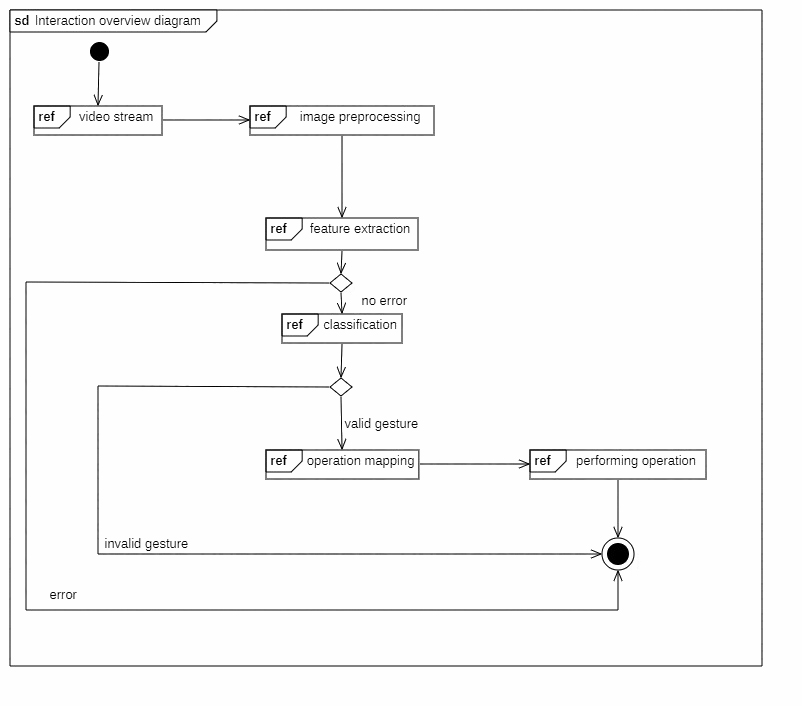
\includegraphics[width=\textwidth]{Image/Interaction overview diagram.jpg}}
        	  \caption{Interaction overview diagram}
        	  \label{fig:Interaction overview diagram}
        	\end{figure}
        \end{center}
        
        \begin{center}
        	\begin{figure}[!hp]
        		\centering
        		\fbox{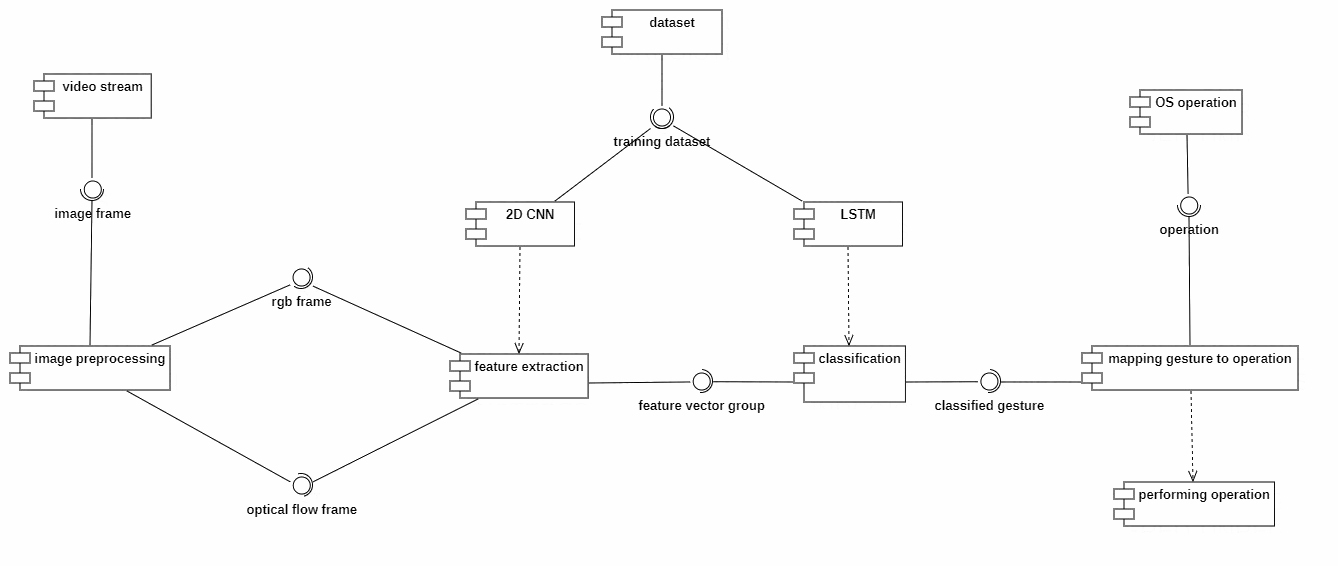
\includegraphics[width=\textwidth]{Image/ComponentDiagram1.jpg}}
        	  \caption{Component diagram}
        	  \label{fig:Component diagram}
        	\end{figure}
        \end{center}
        
        \begin{center}
        	\begin{figure}[!hp]
        		\centering
        		\fbox{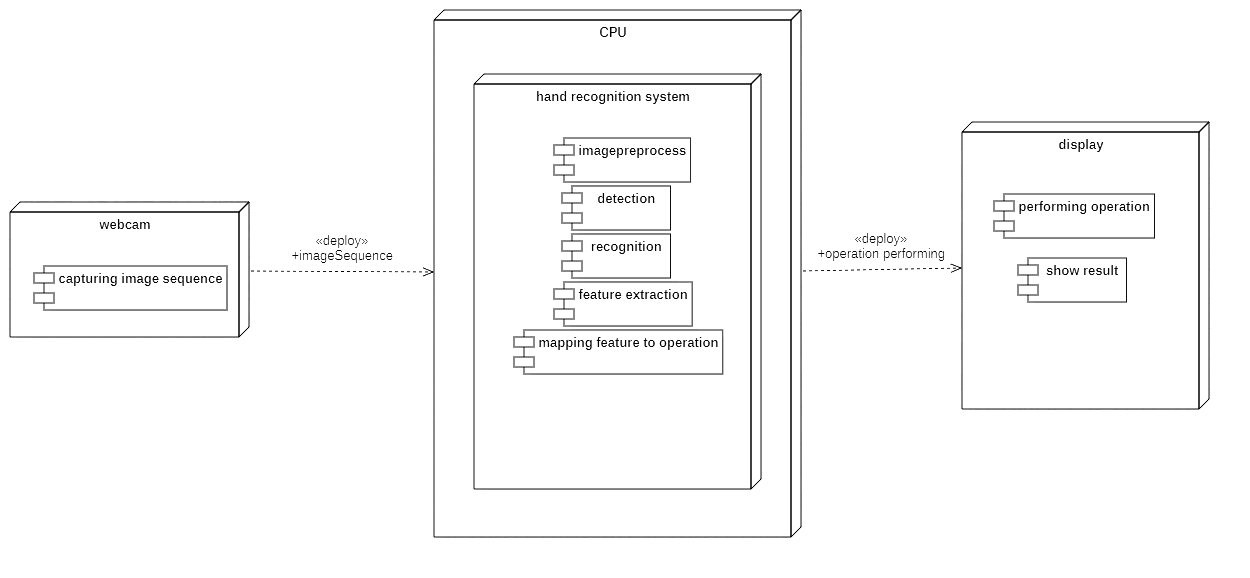
\includegraphics[width=\textwidth]{Image/DeploymentDiagram1.jpg}}
        	  \caption{Deployment diagram}
        	  \label{fig:Deployment diagram}
        	\end{figure}
        \end{center}
        
    
















% \begin{center}
% 	\begin{figure}[!htbp]
% 		\centering
% 		\fbox{\includegraphics[width=\textwidth]{use-case.jpg}}
% 	  \caption{Use case diagram}
% 	  \label{fig:usecase}
% 	\end{figure}
% \end{center} 
















\chapter{OTHERS SPECIFICATION}

    \section{Advantages}
    Through this system we can establish basic system control without actually having to
come in contact with the system physically.
    The mode of input, i.e., video tracking, can potentially make the computation quite
intensive; but the algorithm used for classification of gestures tries to handle it such
that the process does not become too computationally draining.

    \section{Limitations}
        . The system may take a considerable amount of time(say, a few seconds) to correctly
classify the gesture made based on how the algorithm is trained. This can cause a
delay in the intended operation that is to be performed.
    The system, as simple as it might be made to be, might still not be as intuitive to some
users. So, some literacy on how to use such systems needs to be provided.
    The hand gestures made by one particular user may vary significantly in comparison
to those made by another user; this is more of a subjective choice as to how a
particular user thinks and can be difficult to generalize. It might occur that the
particular set of gestures that the system is trained to classify might be different to
what a user actually performs.

\section{Applications}
    The hand gesture recognition system can be employed in public systems, such as an
automated teller machine(ATM) where potentially scores of people might handle the
same interface through physical touch. This can potentially prevent the spread of any
physical contact-intensive diseases.
    The system can potentially help to achieve truly contact-less operation at an even
greater scale, such as workplaces where employees interact with a common interface
through physical touch, albeit through objects like ID cards; or supply chain workers
who might handle the same interface throughout the day.














\chapter{CONCLUSION AND FUTURE WORKS}
In future we can map more gesture to different navigation operation which can we user more control of the screen. And we can decrease the latency by increasing the training dataset and Neural Network nodes.















\end{appendices}


\end{document}
